\documentclass[oneside,bibliography=totoc,openany]{scrbook}
%\setcounter{secnumdepth}{0}
%\usepackage{showframe}
\usepackage{amsmath,amssymb}
\numberwithin{figure}{section}
\numberwithin{table}{section}
\makeatletter
\newcommand{\mathleft}{\@fleqntrue\@mathmargin0pt}
\newcommand{\mathcenter}{\@fleqnfalse}
\makeatother
\usepackage{enumerate}
\usepackage{geometry}
\usepackage{ifoddpage}
\usepackage{calc}
\usepackage{lipsum}
\usepackage{changepage}
\usepackage{graphicx}
\usepackage{blindtext}
\usepackage[bottom]{footmisc}
\usepackage[ngerman]{babel}
\usepackage{wrapfig}
\usepackage{float}
\usepackage{titletoc}
%\restylefloat{table}
%\usepackage{sidenotes}
%\usepackage{mwe}
\usepackage[utf8]{inputenc}

%custom packages not from template
\usepackage{silence}
\WarningFilter{scrbook}{Usage of package `fancyhdr'}
%end of custom packages not from template

\usepackage[bookmarks,hypertexnames=false,debug,hidelinks]{hyperref}
\usepackage{bookmark}
\usepackage{nameref} 
\usepackage[listformat=empty]{caption}
\captionsetup{justification=raggedright,singlelinecheck=false}
\usepackage{marginnote}
\usepackage[export]{adjustbox}
%\usepackage{tocloft}
%\renewcommand{\cftchapleader}{\cftdotfill{\cftdotsep}}
%\renewcommand{\cftsecleader}{\cftdotfill{\cftdotsep}}
\usepackage{fancyhdr}
\usepackage{frutiger}
\usepackage{lmodern}
%\setlength{\cftfignumwidth}{-15pt}
%\setlength{\cfttabnumwidth}{-15pt}
%\DeclareCaptionType{formel}[][Formelverzeichnis]
%\captionsetup[formeln]{labelformat=empty}

%custom packages not from template
\usepackage{scrhack}
\usepackage[newfloat]{minted}
\addto\captionsngerman{%
  \renewcommand{\listlistingname}{Quellcodeverzeichnis}%
  \renewcommand{\listingname}{Quellcode}%
}
\usepackage{microtype}
\usepackage[capitalise,ngerman]{cleveref}
\addto\captionsngerman{
    % Second argument is singular, third is plural
    \crefname{listing}{Quellcode}{Quellcodes}
    \Crefname{listing}{Quellcode}{Quellcodes}
}

\usepackage{csquotes}
\MakeOuterQuote{"}

\usepackage[onehalfspacing]{setspace} 
%end of custom packages not from template
\usepackage[style=numeric,citestyle=numeric,backref=true,urldate=long,backend=biber]{biblatex}
\geometry{top=25mm, left=20mm, right=30mm, bottom=20mm}
\setlength{\marginparwidth}{10mm}

\newlength{\tempParIndent}
\newcommand{\textBody}[1]{%
    \begin{minipage}[t]{\linewidth-5cm-\marginparsep}
    \setlength{\parindent}{\tempParIndent}%
        #1
    \end{minipage}%
    }
\newcommand{\noteBody}[1]{%
    \begin{minipage}[t]{50mm}
        #1
    \end{minipage}%
}
\newcommand{\textAndNote}[2]{%
    % input:
    % #1: The main text
    % #2: The note
    \setlength{\tempParIndent}{\parindent}
    \begin{adjustwidth*}{}{-\marginparwidth-\marginparsep}%
    \checkoddpage%
\ifoddpage%
    \textBody{#1}%
    \hspace{\marginparsep}%
    \noteBody{#2}%
\else%
    \noteBody{#2}%
    \hspace{\marginparsep}%
    \textBody{#1}%
\fi%
    \end{adjustwidth*}}

\addbibresource{literatur.bib}

\begin{document}

\thispagestyle{plain}

\begin{titlepage}

    \begin{flushleft}

        \begin{center}

            \LARGE{{\textbf{Fehlersuche und Visualisierung der Belegung von Synchronisationsmitteln
            in nebenläufigen Systemen}}}\\[1.5ex]
            \Large{\textbf{}}\\[12ex]
            \Large{\textbf{Bachelorarbeit}}\\[1.5ex]

            \large{FernUniversität in Hagen}\\
            \large{Fakultät für Mathematik und Informatik}\\[48ex]
            
        \end{center}

        \normalsize{}
        \begin{tabular}{ll}
            vorgelegt von:  & \quad Marcel Sobottka\\[1.2ex]
            Matrikelnummer: & \quad 8989265\\[1ex]
            Erstgutachter:  & \quad Prof.\,Dr.-Ing.\,habil.\,Dr.\,h.c.\,Herwig Unger\\[1ex]
            Betreuer:  & \quad Dipl.-Inform.\,(Univ.)\,Marcel Schaible\\[1ex]
            eingereicht am: & \quad 30.\,April\,2020
        \end{tabular}

    \end{flushleft}

\end{titlepage}

\newpage\null\thispagestyle{empty}\newpage
\cleardoubleoddpage

% \addtocontents{toc}{~\hfill\textbf{Seite}\endgraf}
\pagenumbering{Roman}
\setcounter{page}{3}
\tableofcontents
\thispagestyle{fancy}
% clear all header fields
\fancyhead{} 
%\fancyhead[RO,LE]{\thepage}
\fancyhead[R]{\thepage}
\fancyfoot{}
%\addcontentsline{toc}{chapter}{Inhaltsverzeichnis}

\newpage \phantomsection \listoffigures
\thispagestyle{fancy}
% clear all header fields
\fancyhead{} 
%\fancyhead[RO,LE]{\thepage}
\fancyhead[R]{\thepage}
\fancyfoot{}
%\addcontentsline{toc}{chapter}{Abbildungsverzeichnis}

% \newpage \phantomsection \listoftables
% \thispagestyle{fancy}
% % clear all header fields
% \fancyhead{} 
% %\fancyhead[RO,LE]{\thepage}
% \fancyhead[R]{\thepage}
% \fancyfoot{}
% \addcontentsline{toc}{chapter}{Tabellenverzeichnis}

%\newpage \phantomsection
% \listofformel \thispagestyle{fancy} \fancyhead{} clear all header fields
% \fancyhead[RO,LE]{\thepage} \fancyfoot{}
% \addcontentsline{toc}{chapter}{Formelverzeichnis} \newpage

\newpage \phantomsection \listoflistings
%\addcontentsline{toc}{chapter}{Quellcodeverzeichnis}
\addtocontents{lol}{\protect\thispagestyle{fancy}}
\thispagestyle{fancy}
% clear all header fields
\fancyhead{} 
%\fancyhead[RO,LE]{\thepage}
\fancyhead[R]{\thepage}
\fancyfoot{}

\clearpage
\pagenumbering{arabic}  
\setcounter{page}{7}
\parindent 0pt
\fancypagestyle{plain}{%
\fancyhf{}\renewcommand{\headrulewidth}{0pt}}
\pagestyle{fancy}
\renewcommand{\chaptermark}[1]{\markboth{#1}{}}
\renewcommand{\sectionmark}[1]%
{\markboth{#1}{}}
\fancyhead{} % clear all header fields
\fancyhead[RE,LO]{\leftmark}
\fancyhead[RO,LE]{\thepage}
\fancyfoot{}

\startcontents
\chapter{Motivation}
\label{chapter:Motivation}
\thispagestyle{fancy}
\section{Motivation}

Bei der parallelen Programmierung ist die korrekte Verwendung von
Synchronisationsmitteln ein Problem. Während der Entwicklung sind
Nebenläufigkeitsprobleme für den Entwickler nur sehr schwer zu erkennen.
Zusätzlich unterstützen moderne Entwicklungsumgebungen und Compiler den
Entwickler nicht oder nur unzureichend bei diesen Problemen.

Eines dieser Probleme ist das Auftreten von \textit{Deadlocks}, welche in
\cref{section:Deadlockerkennung allgemein} beschrieben werden.
Das grundlegende Verfahren zur Identifizierung von potenziellen Deadlocks
ist in \cref{section:Deadlockerkennung allgemein} beschrieben. Anschließend
werden in \cref{section:Evaluierung von Methoden zur dynamischen
Deadlockerkennung} zwei Verfahren evaluiert. Betrachtet werden Programme die mit
der Echtzeit-Programmiersprache PEARL\autocite{PEARL} geschrieben wurden.
 
\stopcontents

\startcontents
\chapter{Analyse}
\label{chapter:Analyse}
\thispagestyle{fancy}
\printcontents{l}{1}{\setcounter{tocdepth}{5}}
\section{Deadlockerkennung allgemein}
\label{section:Deadlockerkennung allgemein}
Im Gegensatz zu Single-Threaded-Applikationen sind Multi-Threaded-Anwendungen
nicht deterministisch. Dies kann zu \textit{race conditions} führen. Eine
\textit{race condition} tritt zum Beispiel dann auf, wenn zwei Threads einen
Zähler jeweils um eins erhöhen wollen. Angenommen der Zähler hat zu Beginn den
Wert drei. Beide Threads wollen jetzt nahezu gleichzeitig den Zähler um eins
erhöhen. Dazu lesen beide Threads den aktuellen Wert des Zählers, in diesem Fall
drei, aus. Anschließend addieren beide eins hinzu und schreiben den neuen Wert,
in diesem Fall vier, in den Zähler. Erwartet wurde jedoch der Wert fünf, da
beide Threads den Zähler um jeweils eins erhöhen sollten. Um solche \textit{race
conditions} zu verhindert werden Synchronisierungsmechanismen benötigt.

Eine Möglichkeit um den Zugriff auf eine gemeinsame Ressource zu synchronisieren
sind Locks. Ein Lock ist ein exklusiver Zugriff auf ein Objekt, ein sogenanntes
Lockobjekt. Das bedeutet, dass während ein Thread einen Lock auf ein Objekt
besitzt, andere Threads, welche auf dasselbe Objekt zugreifen wollen, warten
müssen bis es freigegeben wurde.

Betrachtet man das Beispiel mit dem Zähler erneut, dieses Mal mit Locks als
Synchronisationsmittel, kann es zu folgender Ausführung kommen. Der Zähler hat
zu Beginn wieder den Wert drei. Die Threads \textit{T1} und \textit{T2} wollen
erneut den Zähler nahezu gleichzeitig erhöhen. Dieses Mal versuchen beide das
Lockobjekt \textit{L1} in Besitz zu nehmen. Der Thread \textit{T2} nimmt
\textit{L1} zuerst in Besitz, daraus folgt \textit{T1} muss warten. \textit{T2}
liest den aktuellen Wert des Zählers aus, erhöht diesen um eins und schreibt den
neuen Wert vier in den Zähler. Anschließend gibt \textit{T2} das Lockobjekt
\textit{L1} frei. Jetzt erhält der Thread \textit{T1} den Zugriff auf
\textit{L1} und liest ebenfalls den Zähler, jetzt vier, aus, erhöht diesen und
schreibt den neuen Wert fünf in den Zähler. Anschließend gibt \textit{T1} das
Lockobjekt \textit{L1} frei.

Die Verwendung von Locks in Verbindung mit der nicht deterministischen
Ausführung von Multi-Threaded-Anwendungen, kann zu folgender Situation führen:
Angenommen es existieren zwei Threads \textit{T1} und \textit{T2} und zwei
Lockobjekte \textit{L1} und \textit{L2}. Angenommen \textit{T1} besitzt
\textit{L1} und zu gleichen Zeit erlangt \textit{T2} das Lockobjekt \textit{L2}.
Wenn jetzt der Thread \textit{T1} das Lockobjekt \textit{L2} anfordert und der
Thread \textit{T2} das Lockobjekt \textit{L1}, kommt es zu einem
\textit{Deadlock}. Die Ausführung des Programms terminiert nicht, da beide
Threads auf den jeweils anderen Thread warten und sich gegenseitig blockieren.

Solche potenziellen Deadlocks zu erkennen ist die Aufgabe von statischen und
dynamischen Methoden zur Deadlockerkennung. Die statische Deadlockerkennung
analysiert den Quellcode und wird hier nicht näher betrachtet. Die dynamische
Deadlockerkennung analysiert eine Anwendung zur Laufzeit und läuft in folgenden
drei Schritten ab:
\begin{enumerate}
  \item Erstellung einer Trace-Datei
  \item Erstellung eines Graphen basierend auf den Informationen aus der
  Trace-Datei
  \item Finden von potenziellen Deadlocks durch das Identifizieren von Zyklen
  innerhalb des Graphen
\end{enumerate}

Eine Trace-Datei enthält einen \textit{execution trace} des ausführenden
Programms. Ein \textit{execution trace} ist eine Abfolge von Events. Ein Event
\textit{e\textsubscript{i}} wird durch eine der folgenden Methoden definiert:
starten eines Threads, Inbesitznahme eines Lockobjekts und Freigabe eines
Lockobjekts. Das Starten eines neues Threads ist definiert durch:
\begin{quote}
\texttt{s(Programmstelle, ausführender Thread, Name des neuen Threads)}
\end{quote}
Zum Beispiel bedeutet \texttt{s(2,main,T1)}, dass an der Programmstelle
\textit{2} der Thread \textit{main} den Thread \textit{T1} gestartet hat. 
Die Inbesitznahme eines Lockobjekts ist definiert durch:
\begin{quote}
\texttt{l(Programmstelle, ausführender Thread, Name des Lockobjekts)}
\end{quote}
Zum Beispiel bedeutet \texttt{l(24,T1,L3)}, dass
an der Programmstelle \textit{24} hat der Thread \textit{T1} das Lockobjekt
\textit{L3} in Besitz genommen. Die Freigabe eines Lockobjekts ist definiert
durch:
\begin{quote}
\texttt{u(Programmstelle, ausführender Thread, Name des Lockobjekts)}
\end{quote}
Zum Beispiel bedeutet \texttt{u(30, T1, L3)}, dass an der Programmstelle
\textit{30} der Thread \textit{T1} das Lockobjekt \textit{L3} freigegeben hat.

Die Menge aller während der Laufzeit des Programms aufgetretenen Events
definieren einen möglichen \textit{execution trace} des Programms.
Programme welche mit mehreren Threads arbeiten, haben keinen deterministischen
\textit{execution trace}. Jede Ausführung eines solchen Programms kann zu
unterschiedlichen \textit{execution traces} führen. 

Im zweiten Schritt wird aus dem vorher erzeugten \textit{execution trace} ein
Lockgraph erstellt. Ein Lockgraph ist definiert durch:
\begin{quote}
\textit{LG = (L,R)}
\end{quote}
\textit{L} ist die Menge aller Lockobjekte im \textit{execution trace} und
\textit{R} die Menge aller Lockpaare. Ein Lockpaar ist definiert durch das Tupel
\textit{(l\textsubscript{1}, l\textsubscript{2})} für das gilt: Es existiert ein
Thread, welcher das Lockobjekt \textit{l\textsubscript{1}} besitzt, während er
den Lock \textit{l\textsubscript{2}} anfordert.

\section{PEARL}
\label{section:PEARL}
\begin{itemize}
    \item Kurze Beschreibung der Programmiersprache PEARL
    \item Aufzeigen der Möglichkeiten von Synchronisationsmitteln in PEARL
\end{itemize}

\begin{listing}[ht]
  \inputminted[frame=lines,linenos]{vim}{./Examples/Example_Deadlock.prl}
  \caption{Beispiel einer OpenPEARL Anwendung mit einem potenziellen Deadlock}    
  \label{lst:ExampleDeadlock}   
\end{listing} 

In \cref{lst:ExampleDeadlock} ist ein Beispielprogramm in der Programmiersprache
PEARL dargestellt. Das Programm startet zwei parallele Aufgaben welche beide eine Zeichenfolge auf der Standardausgabe ausgeben. Der Zugriff auf die Standardausgabe muss dabei synchronisiert erfolgen.

In den Zeilen 1 bis 11 werden Variablen definiert, wie zum Beispiel die Ausgabe über die Standardausgabe und die zwei \textit{SEMA} Variablen \textit{L1} und \textit{L2} in den Zeilen 9 und 10. Ein \textit{SEMA} Objekt ist ein Semaphore und dient als Synchronisationsmittel. Es kann als Wert nicht negative ganze Zahlen besitzen, wobei null den Zustand "gesperrt" und positive Zahlen den Zustand "frei" bedeuten \autocite[9--17]{PEARL}. Eine \textit{SEMA} Variable hat zu Beginn den Wert null und den Zustand "gesperrt". In den Zeilen 12 bis 17 ist ein \textit{TASK} definiert. Durch die Kennzeichnung \textit{MAIN} wird der \textit{TASK} direkt beim Start des Programms ausgeführt. Die Befehle \textit{RELEASE} in den Zeilen 13 und 14 erhöhen den Wert der jeweiligen \textit{SEMA} Variable um eins, wodurch der Zustand von "gesperrt" auf "frei" gesetzt wird. Anschließend werden in den Zeilen 15 und 16 die \textit{TASKS} \textit{T2} und \textit{T3} gestartet.

Die \textit{TASKS} \textit{T2} und \textit{T3} geben in den Zeilen 22 bis 24 und in den Zeilen 32 bis 34 die Zeichenfolge "Hello World T2" bzw. "Hello World T3" auf der Standardausgabe aus. Die Synchronisierung des Zugriffs auf die Standardausgabe erfolgt mittels den \textit{SEMA} Variablen \textit{L1} und \textit{L2}. Mit dem \textit{REQUEST} Befehl wird der Wert einer \textit{SEMA} Variable um eins verringert. Ist der Wert einer \textit{SEMA} Variable null wird der \textit{TASK} angehalten und in eine Warteschlange eingereiht. Sobald die Variable über den Befehl \textit{RELEASE} wieder freigeben wird, wird der nächste \textit{TASK} in der Warteschlange gemäß seiner Priorität fortgeführt. Beide \textit{TASKS} versuchen beide \textit{SEMA} Variablen in Besitz zu nehmen. \textit{T2} versucht in den Zeilen 20 und 21 zuerst \textit{L1} und dann \textit{L2} in Besitz zu nehmen. \textit{T3} versucht in den Zeilen 30 und 31 zuerst \textit{L2} und dann \textit{L1} in Besitz zu nehmen. Da beide \textit{TASKS} parallel laufen, kann es passieren, dass \textit{T2} \textit{L1} in Zeile 20 in Besitz nimmt und gleichzeitig \textit{T3} in Zeile 30 \textit{L2} in Besitz nimmt. Beide \textit{SEMA} Variablen haben jetzt den Wert null und den Zustand "gesperrt". Der \textit{TASK} \textit{T2} wartet jetzt darauf, dass \textit{L2} freigegeben wird und \textit{T3} wartet darauf, dass \textit{L1} freigegeben wird. Beide \textit{TASKS} warten auf den jeweils anderen. Diese Situation wird als Deadlock bezeichnet.

\section{MagicLock}
\label{section:MagicLock}
\begin{itemize}
  \item Beschreibung des MagicLock\autocite{MagicLock} Algorithmus
\end{itemize}
\stopcontents

\startcontents
\chapter{Design}
\label{chapter:Design}
\thispagestyle{fancy}
\printcontents{l}{1}{\setcounter{tocdepth}{5}}
\section{Erzeugung der Trace-Datei}
\label{section:Erzeugung der Trace-Datei}
\begin{itemize}
    \item Definition der notwendigen Informationen der Trace-Datei
    \item Aufzeigen der Herausforderungen in Bezug auf Performance und
    Speicherauslastung
  \item Anforderungen definieren:
  \begin{itemize}
    \item Laufzeit des Programms soll sich um maximal x\% erhöhen
    \item Speicherauslastung des Programms soll sich um maximal y\% erhöhen
  \end{itemize}
\end{itemize}

\section{Analysieren der Trace-Datei}
\label{section:Analysieren der Trace-Datei}
\begin{itemize}
  \item Externes Programm geschrieben in Java
  \item Anforderungen definieren:
  \begin{itemize}
    \item Darstellung der Trace-Datei (welcher Thread hat welches
    Synchronisationsmittel wann genommen und wieder freigegeben) 
  \end{itemize}
\end{itemize}

\section{Erweiterung: Potenzielle Deadlocks}
\label{section:Erweiterung: Potenzielle Deadlocks}
\begin{itemize}
  \item Programm aus \cref{section:Analysieren der Trace-Datei} wird erweitert
  \item Es sollen potenzielle Deadlocks mit Hilfe des aus \cref{section:MagicLock}
 beschriebenen Verfahrens bestimmt werden
  \item Potenzielle Deadlocks sollen als gerichtete Graphen visualisiert werden
\end{itemize}
\stopcontents

\startcontents
\chapter{Implementierung}
\label{chapter:Implementierung}
\thispagestyle{fancy}
\printcontents{l}{1}{\setcounter{tocdepth}{5}}
\section{Trace Funktion}\label{Implementierung:Trace Funktion}
\begin{itemize}
  \item Vorstellung der Implementierung der Trace Funktionalität in PEARL
\end{itemize}

\section{Analyse Programm}
\begin{itemize}
  \item Vorstellung der Implementierung des Analyse Programms in Java
  \item Grafiken/Screenshots mit Analyse Beispielen
\end{itemize}

\section{Visualisierung von potenziellen Deadlocks}
\begin{itemize}
  \item Vorstellung der Implementierung des Algorithmus zur Erkennung von
  potenziellen Deadlocks
  \item Grafiken/Screenshots mit Analyse Beispielen
\end{itemize}
\stopcontents

\startcontents
\chapter{Validierung}
\label{chapter:Validierung}
\thispagestyle{fancy}
\printcontents{l}{1}{\setcounter{tocdepth}{5}}
\section{Trace Funktion}\label{Validierung:Trace Funktion}
\begin{itemize}
  \item Beispielprogramme in PEARL definieren
  \item Anforderungen validieren:
  \begin{itemize}
    \item Laufzeiten der einzelnen Programme mit und ohne Trace Funktionalität
    bestimmen und vergleichen, mit Python Programm
    \cref{lst:Python_Benchmark_CPU}
    \item Speicherauslastung der einzelnen Programme mit und ohne Trace
    Funktionalität bestimmen und vergleichen, mit Python Programm
    \cref{lst:Python_Benchmark_Memory}
  \end{itemize}
\end{itemize}

\begin{listing}[ht]
  \inputminted[frame=lines,linenos]{python}{./Python/benchmark_cpu.py}
  \caption{Pythonskipt zur Messung der Laufzeit}
  \label{lst:Python_Benchmark_CPU}   
\end{listing} 

\begin{listing}[ht]
  \inputminted[frame=lines,linenos]{python}{./Python/benchmark_memory.py}
  \caption{Pythonskipt zur Messung der Speicherauslastung}
  \label{lst:Python_Benchmark_Memory}   
\end{listing} 

\section{Analyse Programm}
\label{section:ValidierungAnalyseProgramm}
Für die chronologische Darstellung der Lockobjekte wird die Trace-Datei aus
\cref{lst:ExampleTraceFile} mit drei Threads und neun Lockobjekten.
\begin{listing}[ht]
  \begin{minipage}[ht]{\linewidth}
    \begin{multicols}{3}
      \inputminted[linenos]{text}{./Examples/ExampleTraceFile.log}
    \end{multicols}
    \caption{Beispielhafte Trace-Datei mit einem potenziellen Deadlock}
    \label{lst:ExampleTraceFile}
  \end{minipage}
\end{listing}
In dem Beispiel gibt es zusätzlich zwei Einträge mit dem gleichen Zeitstempel in
den Zeilen 3 und 4 sowie in den Zeilen 13 und 14. Die Ausgabe der Anwendung aus
\cref{section:Implementierung:Analyse Programm} ist in
\cref{fig:LockTraceVisualization} dargestellt.
\begin{figure}[ht]
  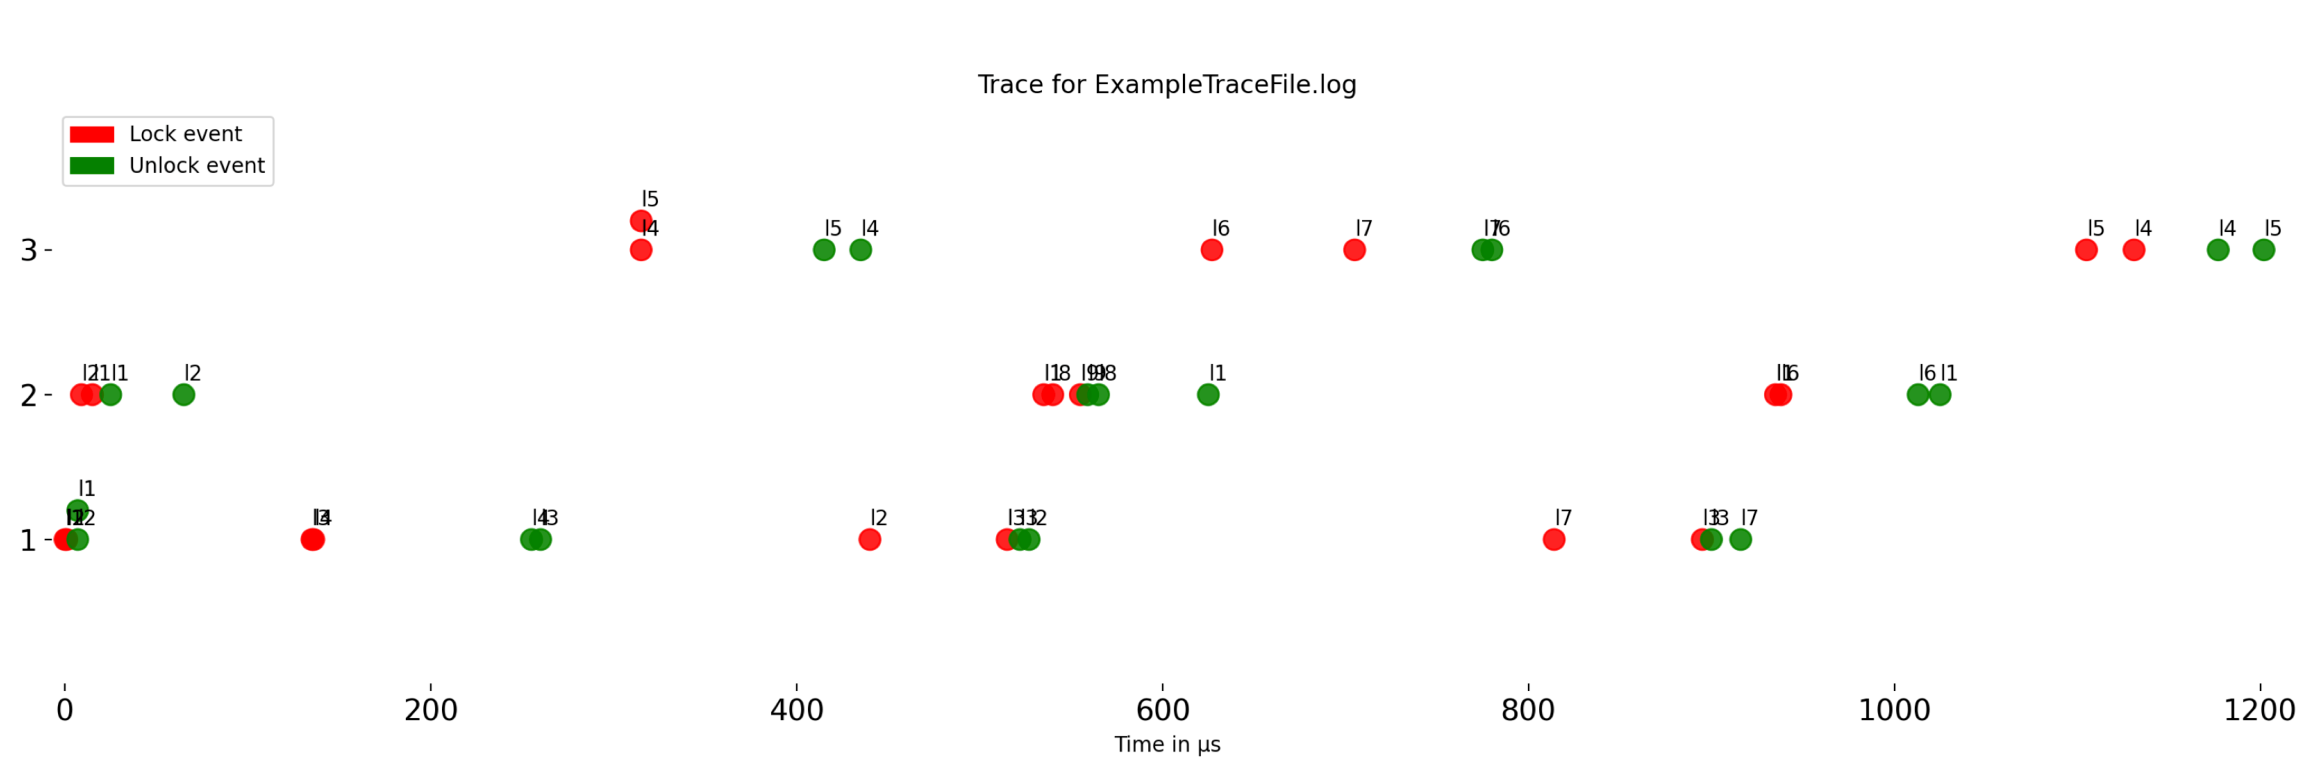
\includegraphics[width=\linewidth]{ExampleTraceFile.eps}
  \caption{Ausgabe der Analyse-Anwendung}
  \label{fig:LockTraceVisualization}
\end{figure}
Die überlappenden Logeinträge können auseinander gezogen werden in dem in den
Graphen hineingezoomt wird. Wird zum Beispiel auf die ersten 70 Mikrosekunden
vergrößert, werden die Logeinträge auseinander gezogen siehe
\cref{fig:LockTraceVisualizationZoomed}.
\begin{figure}[ht]
  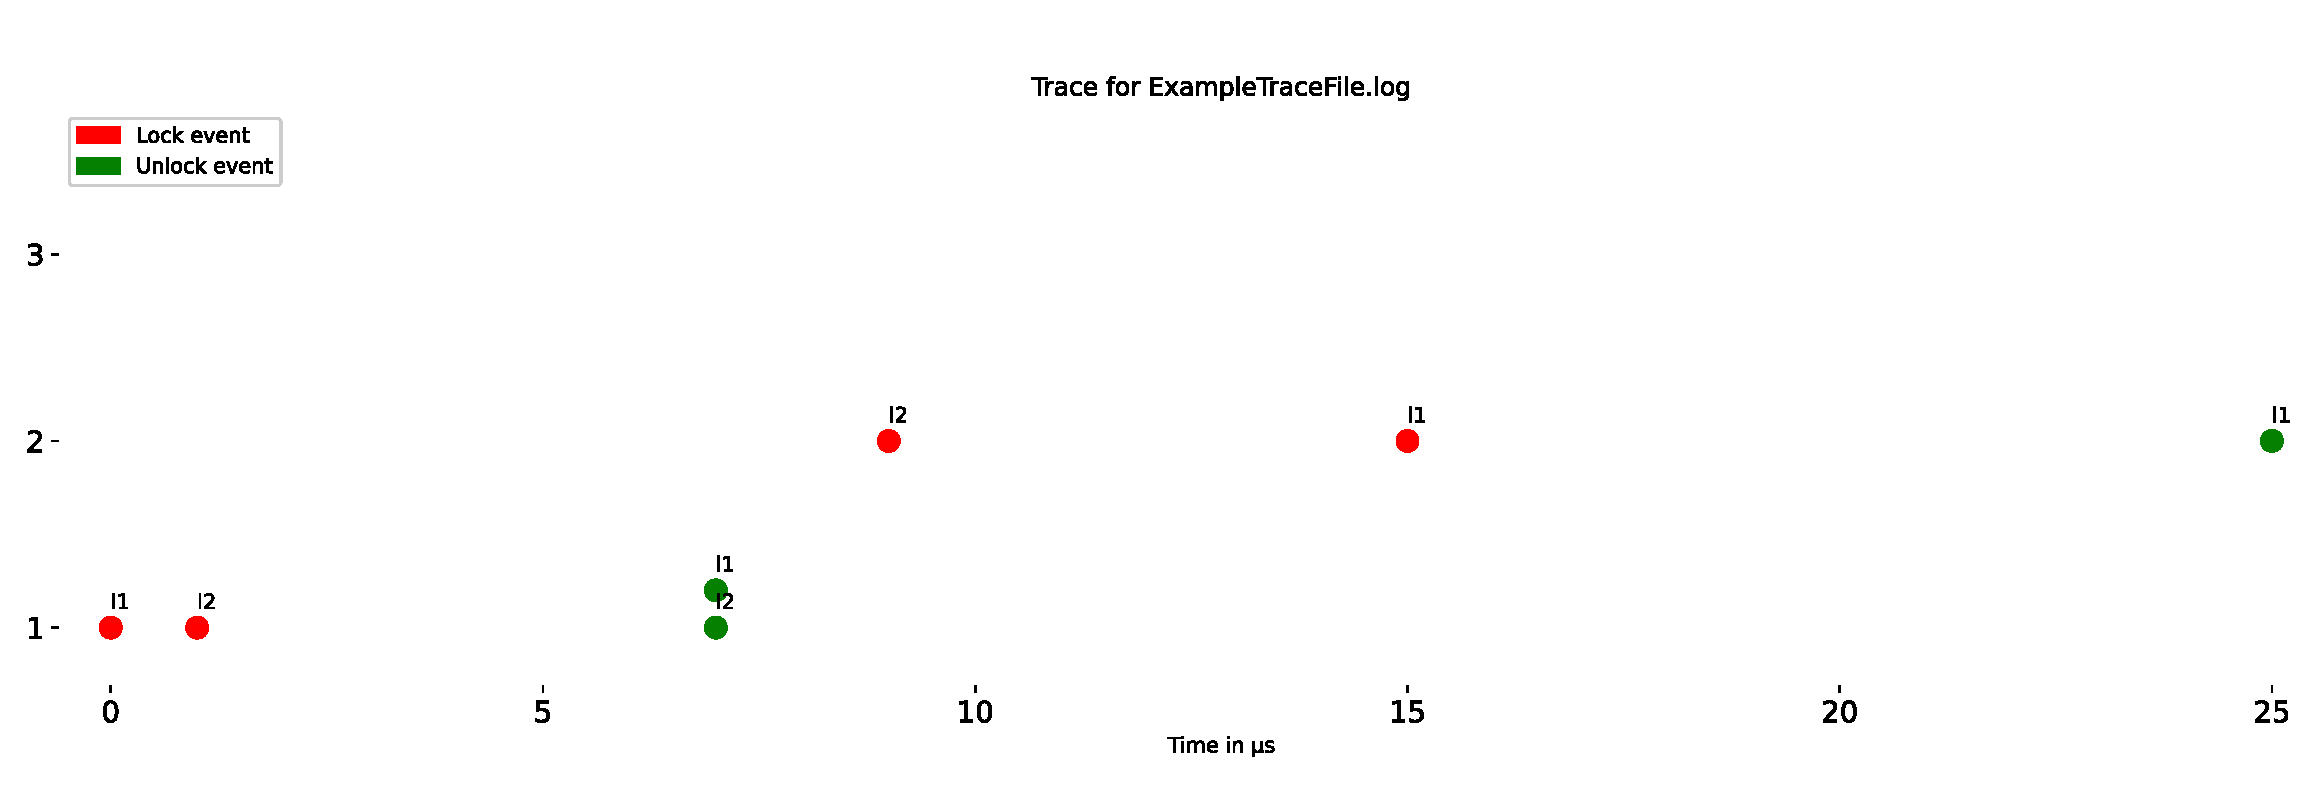
\includegraphics[width=\linewidth]{ExampleTraceFileZoomed.eps}
  \caption{Vergrößerte Darstellung von \cref{fig:LockTraceVisualization}}
  \label{fig:LockTraceVisualizationZoomed}
\end{figure}
Die beiden Logeinträge mit den gleichen Zeitstempel sind bei 7 Mikrosekunden
korrekt vertikal versetzt dargestellt.


\section{Visualisierung von potenziellen Deadlocks}
\label{section:DeadlockVisualization}
Für die Visualisierung von potenziellen Deadlocks wird wieder die Trace-Datei
aus \cref{lst:ExampleTraceFile} verwendet. In dem Beispiel gibt es genau einen
potenziellen Deadlock zwischen den Threads \textit{1} und \textit{2}. In den
Zeilen 1 und 2 nimmt der Thread \textit{1} die Lockobjekten \textit{l1} und
\textit{l2} nacheinander in Besitz. In den Zeilen 5 und 6 nimmt der Thread
\textit{2} die Lockobjekte \textit{l2} und \textit{l1} nacheinander in Besitz.
Der potenzielle Deadlock entsteht, da der Thread \textit{1} zuerst das
Lockobjekt \textit{l1} in Besitz nehmen kann und bevor dieser das Lockobjekt
\textit{l2} in Besitz nehmen kann, kann der Thread \textit{2} das Lockobjekt
\textit{l2} bereits in seinen Besitz genommen haben. Dadurch blockieren sich
beide Threads gegenseitig und ein Deadlock entsteht. Die Ausgabe der Anwendung
zur Erkennung und Visualisierung von potenziellen Deadlocks ist in
\cref{fig:DeadlockVisualization} dargestellt.
\begin{figure}[ht]
  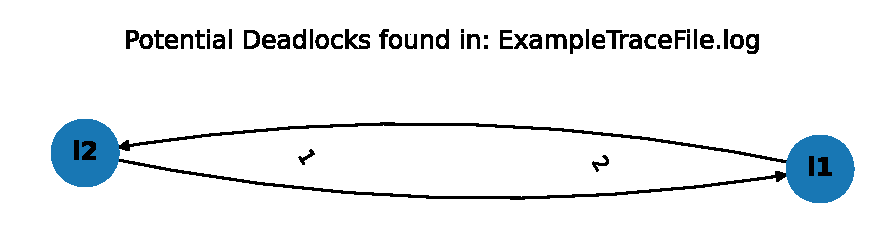
\includegraphics[width=\linewidth]{ExamplePotentialDeadlocks.eps}
  \caption{Ergebnis der Erkennung von potenziellen Deadlocks aus \cref{lst:ExampleTraceFile}}
  \label{fig:DeadlockVisualization}
\end{figure}
Die Beschriftung der Kanten erfolgt immer zum Ende der Kante hin, zum Beispiel
gehört die Beschriftung \textit{1} zu der Kante von \textit{l1} zu \textit{l2}.
Zusätzlich zur grafischen Darstellung werden die Ergebnisse als
Zyklische-Lock-Dependency-Chain auf der Konsole ausgegeben. Für die verwendete
Trace-Datei wird "(1,l2,{l1}) (2,l1,{l2})" als potenzieller Deadlock auf der
Konsole ausgegeben.
\stopcontents

\startcontents
\chapter{Ausblick}
\label{chapter:Ausblick}
\thispagestyle{fancy}
\printcontents{l}{1}{\setcounter{tocdepth}{5}}
\section{Offene Punkte}
\begin{itemize}
  \item Aufzeigen was nicht gemacht wurde und warum (eventuell welche
  Synchronisationsmittel nicht erkannt werden (nur Sema keine Bolt Variablen))
\end{itemize}

\section{Weiterentwicklung}
\begin{itemize}
  \item Alle möglichen Synchronisationsmittel erkennen
  \item Trace Funktionalität in den OpenPEARL Compiler integrieren, so dass es
  mittels compiler flag an und ausgeschaltet werden kann
\end{itemize}
\stopcontents


\printbibliography

\end{document}